%
% fig/hybrid.tex -- Übergang Quadtree -> Newton
%
\begin{figure}
\centering
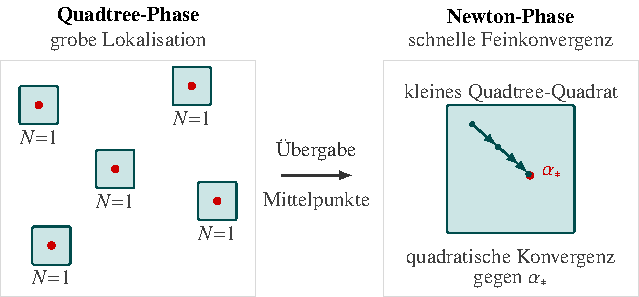
\includegraphics{papers/weyl/images/hybrid.pdf}
\caption{Hybrid-Strategie: links liefert der Quadtree-Algorithmus für jede Nullstelle
ein kleines Quadrat mit $N(D_i) = 1$, das nur noch eine einzige Nullstelle enthält.
Die Mittelpunkte dieser Quadrate dienen als Startwerte $z_0$ für das
Newton-Verfahren (rechts), das in wenigen Schritten quadratisch gegen die wahre
Nullstelle $\alpha_*$ konvergiert. So vereinen sich die globale Zuverlässigkeit des
Quadtree und die lokale Geschwindigkeit von Newton.
\label{weyl:fig:hybrid}}
\end{figure}
